\documentclass{article}
\usepackage{graphicx} % Required for inserting images
\usepackage{float}
\usepackage[T1]{fontenc}
\usepackage{amsmath}
\usepackage[margin=1in]{geometry}
\usepackage{booktabs}
\usepackage{tabularx}
\usepackage[hidelinks]{hyperref}

\title{Running the signal hourly, or at another time of day, on the SPY gamma book}
\author{Experiment report \textperiodcentered{} L/S Gamma Desk, QUANTT}
\date{2026-10-21}

\begin{document}

\maketitle

\textbf{Question:} Does running the daily loop (signal, exits, entry, delta hedge) every hour from 10:15 to 15:15 ET, instead of once at 10:15, make more entries? And does one run a day at another time (12:45 or 15:45) make more entries?

\textbf{Method:}

\begin{itemize}

\item \textbf{Pre-registration:} the hypothesis card, config and script were committed before any run (commit 2784f7c). No engine code was added.

\item \textbf{Data:} the paper rules (\texttt{configs/\allowbreak{}paper.\allowbreak{}toml}: both sides, ATM option, 1-share hedge threshold) are replayed on R2 replay snapshots v1 (config\_hash b040760187f0) over the development window 2014-06-02 to 2024-12-31. The hold-out (2025-01-01 to 2026-07-10) was not used.

\item \textbf{Variants:} only \texttt{[schedule]} changes. \texttt{hourly} (primary): signal and hedge at 10:15, 11:15, 12:15, 13:15, 14:15 and 15:15. \texttt{midday}: one run at 12:45. \texttt{close}: one run at 15:45. Each run checks exits, enters if no position is open and the signal is long or short, then delta-hedges. This is what the live runner does on each run, so \texttt{hourly} also hedges and checks stops six times a day.

\item \textbf{Timing:} every run decides on data 15 minutes old and fills on trades in the next 15 minutes. Spot comes from put-call parity on the 30-minute grid (10:15 to 15:45). The GARCH forecast uses completed days only, so it is the same at every run of a day; only the ATM implied volatility changes during the day.

\item \textbf{Comparison:} the registered baseline (trial 1: one run a day at 10:15), at the same spread multiple.

\item \textbf{Runs:} every variant ran once at 1x and 2x spreads. Costs are \$0.65 per contract and \$0.005 per share, with a \$1 minimum per order.

\end{itemize}

This report was written by Claude at the PM's request.

\section{Result vs the pass bar}

The PM set an entries-only bar: \texttt{hourly} must make more round trips than the baseline over the full window and in each half, with a daily tail (ES 5\%, the mean of the worst 5\% of daily P\&L, USD for one contract) no more than 10\% worse. Every check had to hold at 1x and 2x. Entries are counted as round trips; the last development position is closed by the embargo, so every entry has an exit.

\begin{center}\small
\begin{tabularx}{\linewidth}{>{\raggedright\arraybackslash}X l l l l l}
\toprule
\textbf{Check (\texttt{hourly} vs baseline)} & \textbf{1x value} & \textbf{1x bar} & \textbf{2x value} & \textbf{2x bar} & \textbf{Result} \\
\midrule
Round trips, full window & 225 & > 131 & 225 & > 131 & pass \\
Round trips, 2014-06 to 2019-12 & 92 & > 44 & 92 & > 44 & pass \\
Round trips, 2020-01 to 2024-12 & 133 & > 87 & 133 & > 87 & pass \\
abs ES 5\% \ensuremath{\leq} 1.10 \ensuremath{\times} baseline & 85.6 & \ensuremath{\leq} 106.1 & 94.3 & \ensuremath{\leq} 115.0 & pass \\
\bottomrule
\end{tabularx}
\end{center}

\textbf{Verdict: passed.} Hourly runs make 72\% more round trips (225 against 131), more in both halves, with a smaller daily tail. But the book loses more money: net P\&L is \ensuremath{-}\$3,848 against \ensuremath{-}\$2,060 at 1x, and \ensuremath{-}\$6,705 against \ensuremath{-}\$4,122 at 2x. Net P\&L was reported, not part of the bar.

The same four checks were applied to the single-time variants as a secondary result, as pre-registered. Neither passes:

\begin{center}\small
\begin{tabularx}{\linewidth}{>{\raggedright\arraybackslash}X l >{\raggedright\arraybackslash}X >{\raggedright\arraybackslash}X}
\toprule
\textbf{Secondary check} & \textbf{Bar} & \textbf{\texttt{midday} (12:45)} & \textbf{\texttt{close} (15:45)} \\
\midrule
Round trips, all & > 131 & 135, pass & 144, pass \\
Round trips, 2014-19 & > 44 & 48, pass & 53, pass \\
Round trips, 2020-24 & > 87 & 87, \textbf{fail} (tie) & 91, pass \\
abs ES 5\%, 1x & \ensuremath{\leq} 106.1 & 91.8, pass & 110.8, \textbf{fail} \\
abs ES 5\%, 2x & \ensuremath{\leq} 115.0 & 99.3, pass & 116.3, \textbf{fail} \\
Result &  & failed & failed \\
\bottomrule
\end{tabularx}
\end{center}

The counts are the same at 1x and 2x.

\subsection{Full-window numbers (not part of the bar)}

\begin{center}\small
\begin{tabularx}{\linewidth}{l l l l >{\raggedright\arraybackslash}X}
\toprule
\textbf{} & \textbf{baseline} & \textbf{hourly} & \textbf{midday} & \textbf{close} \\
\midrule
Net P\&L, 1x & \ensuremath{-}2,060 & \ensuremath{-}3,848 & \ensuremath{-}2,746 & \ensuremath{-}3,504 \\
Net P\&L, 2x & \ensuremath{-}4,122 & \ensuremath{-}6,705 & \ensuremath{-}4,751 & \ensuremath{-}5,543 \\
Sharpe, 1x & \ensuremath{-}0.36 & \ensuremath{-}0.75 & \ensuremath{-}0.52 & \ensuremath{-}0.55 \\
Sharpe, 2x & \ensuremath{-}0.68 & \ensuremath{-}1.25 & \ensuremath{-}0.85 & \ensuremath{-}0.85 \\
Max DD, 1x & 3,027 & 3,928 & 2,918 & 3,855 \\
Max DD, 2x & 4,258 & 6,773 & 4,908 & 5,759 \\
ES 5\%, 1x & \ensuremath{-}96.5 & \ensuremath{-}85.6 & \ensuremath{-}91.8 & \ensuremath{-}110.8 \\
ES 5\%, 2x & \ensuremath{-}104.6 & \ensuremath{-}94.3 & \ensuremath{-}99.3 & \ensuremath{-}116.3 \\
Round trips & 131 & 225 & 135 & 144 \\
Short /\allowbreak{} long & 101 /\allowbreak{} 30 & 183 /\allowbreak{} 42 & 100 /\allowbreak{} 35 & 105 /\allowbreak{} 39 \\
Gross, 1x & \ensuremath{-}986 & +1,581 & \ensuremath{-}1,348 & \ensuremath{-}2,419 \\
Gross, 2x & \ensuremath{-}3,026 & \ensuremath{-}1,232 & \ensuremath{-}3,327 & \ensuremath{-}4,432 \\
Option fees & 262 & 450 & 270 & 288 \\
Hedge fees & 914 & 4,453 & 921 & 939 \\
Hedge orders & 914 & 4,453 & 921 & 939 \\
\bottomrule
\end{tabularx}
\end{center}

Sharpe is on \$250k of paper capital. Gross is round-trip P\&L before commissions (after spreads).

\section{Charts}

\begin{figure}[H]\centering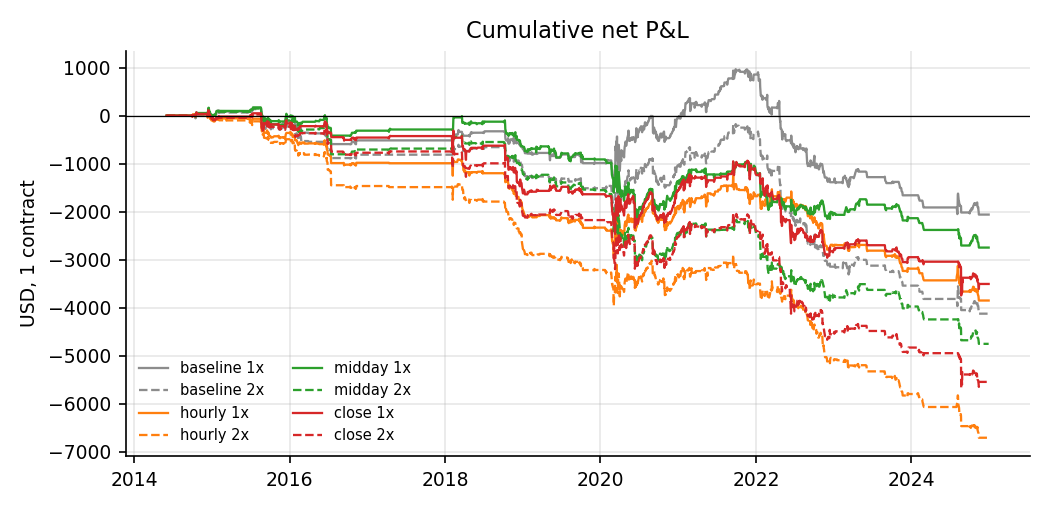
\includegraphics[width=0.92\linewidth]{figures/cum_pnl.png}\caption{Cumulative net P\&L, 1x solid and 2x dashed; baseline grey}\end{figure}

\texttt{hourly} (orange) is below the baseline at 1x on every day from late 2014 on. The gap narrows in 2022, when the baseline loses \$2,242. The baseline's 2020-2021 gain (+\$1,843 at 1x) is mostly missing from every other schedule. \texttt{midday} ends closest to the baseline.

\begin{figure}[H]\centering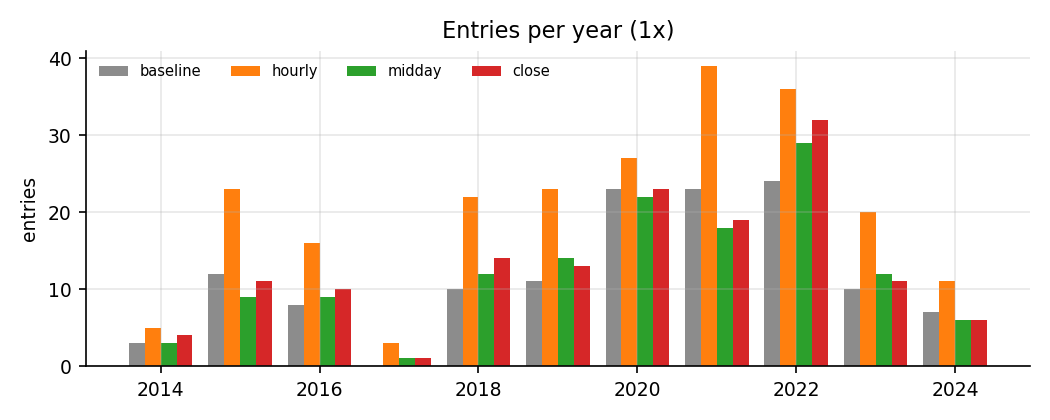
\includegraphics[width=0.92\linewidth]{figures/entries_year.png}\caption{Entries per year, 1x}\end{figure}

\texttt{hourly} makes more entries than the baseline in every year, including 3 in 2017, when the baseline made none. The single-time variants stay close to the baseline each year.

\begin{figure}[H]\centering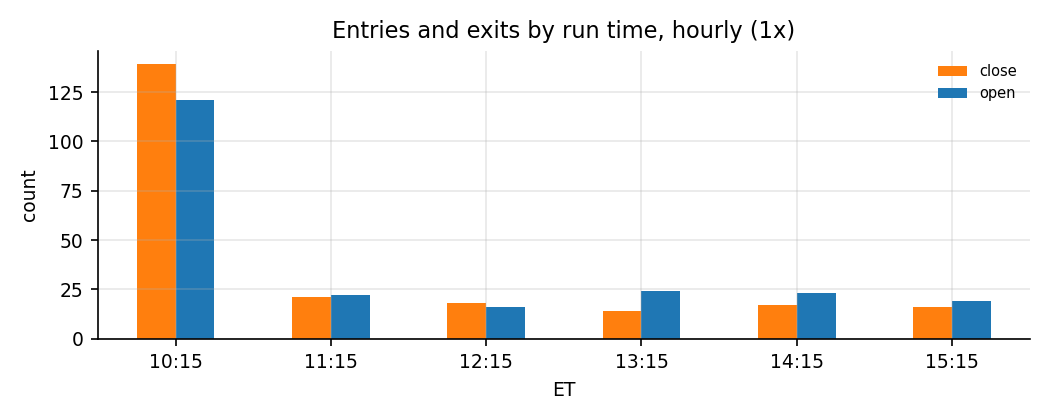
\includegraphics[width=0.92\linewidth]{figures/by_time.png}\caption{Entries and exits by run time, hourly, 1x}\end{figure}

Most hourly entries (121 of 225) still happen at 10:15. The other 104 are spread evenly over 11:15 to 15:15 (16 to 24 per time). Exits follow the same pattern.

\begin{figure}[H]\centering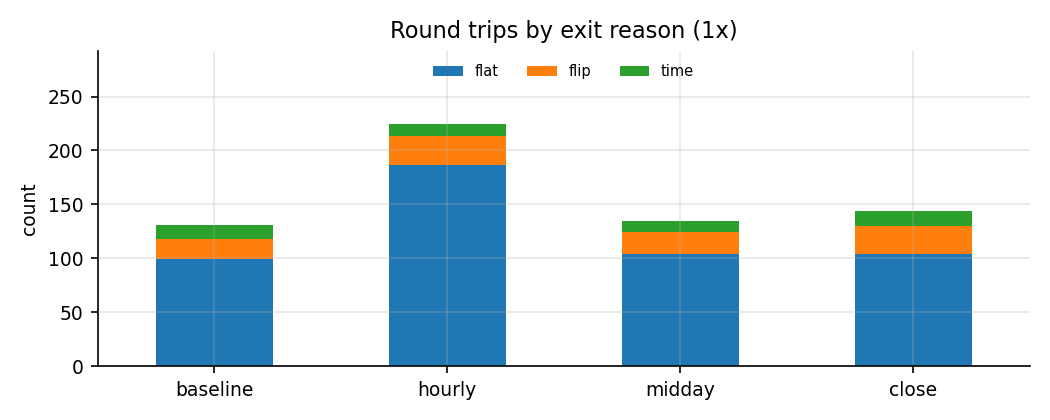
\includegraphics[width=0.92\linewidth]{figures/exits.png}\caption{Round trips by exit reason, 1x}\end{figure}

The extra hourly round trips are almost all flat exits (187 against 99). Flips rise a little (26 against 19) and time exits barely change (12 against 13). No stop or profit-take fired in any variant.

\begin{figure}[H]\centering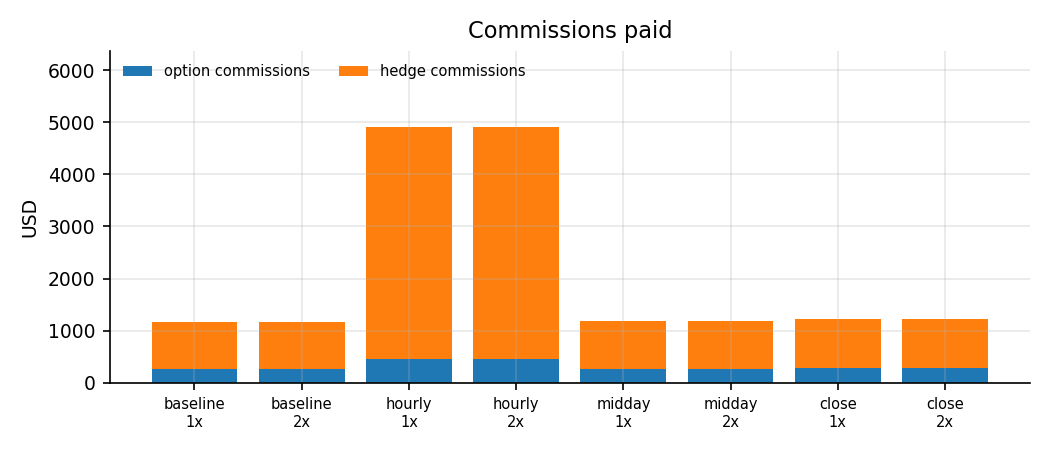
\includegraphics[width=0.92\linewidth]{figures/fees.png}\caption{Commissions paid}\end{figure}

Hedge commissions are almost 5 times the baseline's (\$4,453 against \$914): 4,453 hedge orders at the \$1 minimum each. Option commissions rise with the round trips (\$450 against \$262).

\begin{figure}[H]\centering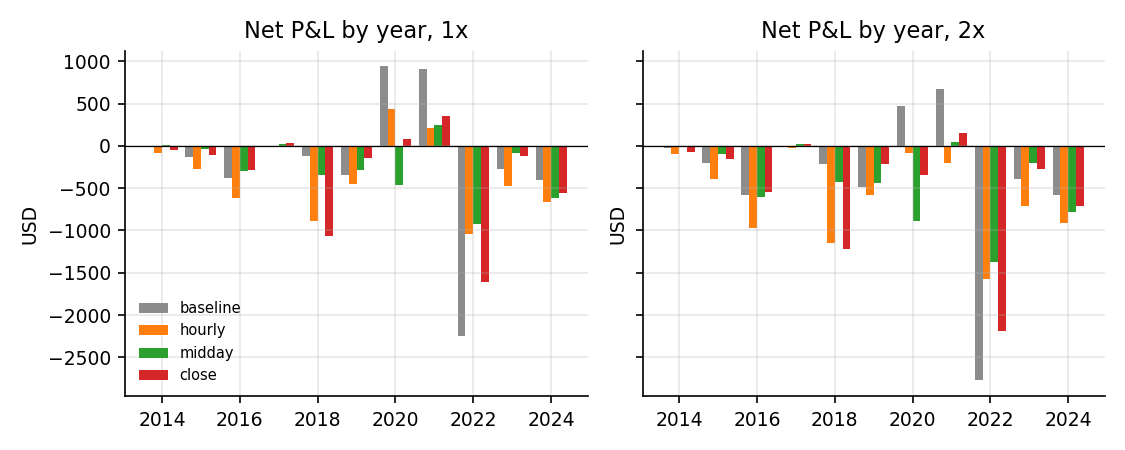
\includegraphics[width=0.92\linewidth]{figures/yearly.png}\caption{Net P\&L by year}\end{figure}

At 1x, \texttt{hourly} does worse than the baseline in 10 of 11 years. The largest gaps are 2018 (\ensuremath{-}\$887 against \ensuremath{-}\$122), 2020 (+\$438 against +\$939) and 2021 (+\$215 against +\$904). The exception is 2022 (\ensuremath{-}\$1,036 against \ensuremath{-}\$2,242).

\begin{figure}[H]\centering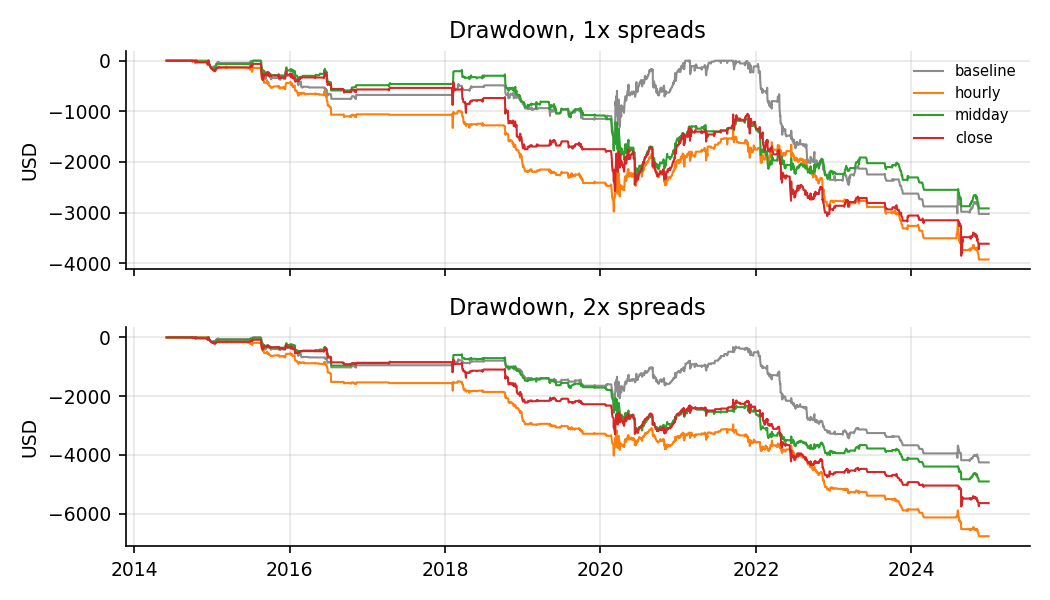
\includegraphics[width=0.92\linewidth]{figures/drawdown.png}\caption{Drawdown at 1x and 2x spreads}\end{figure}

The maximum drawdown rises from \$3,027 to \$3,928 at 1x, and from \$4,258 to \$6,773 at 2x.

\begin{figure}[H]\centering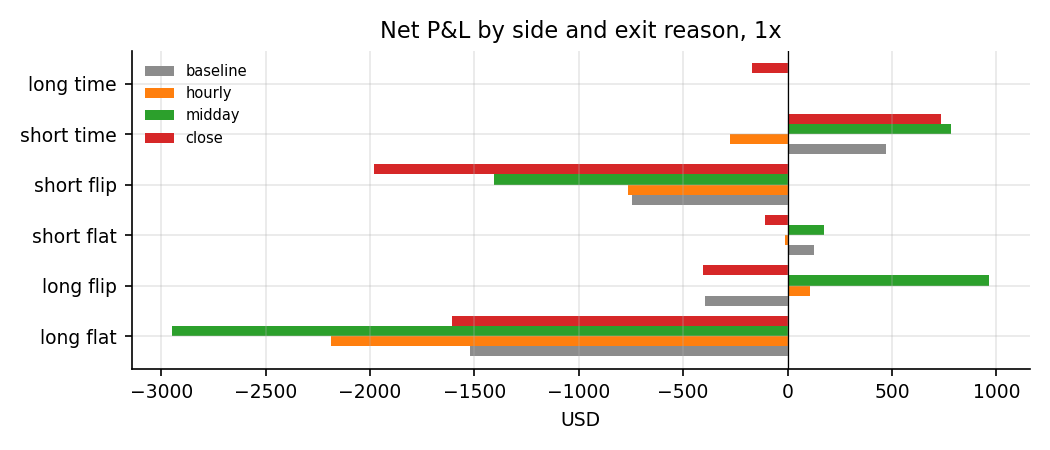
\includegraphics[width=0.92\linewidth]{figures/by_reason.png}\caption{Net P\&L by side and exit reason, 1x}\end{figure}

Longs closed on a flat signal are the largest loss for the baseline, \texttt{hourly} and \texttt{midday}; for \texttt{close} it is short flips (\ensuremath{-}\$1,981). Short flips lose in every schedule. The single-time variants move these buckets by several hundred dollars in either direction, which is consistent with path dependence on few trades.

\section{Analysis}

\textbf{Where the extra hourly entries come from.} \texttt{hourly} makes 94 more round trips than the baseline. 71 of them open and close on the same day, all closed by the flat exit (67 short, 4 long). 45 close one hour after entry. Every one of the 71 follows two days whose last signal was flat. This is mechanical. The 3-day flat exit counts the last signal of each previous day plus the signal of the current run, and an earlier run's signal on the same day is not counted. So when the signal turns short during the day after two flat days, one flat reading at the next run completes the ``three flat days'' and closes the position. With one run a day, a position needs three more flat days before the flat exit can close it. 28 of the 71 opened at 10:15 and closed at a later run that day, which one run a day cannot do. Net of commissions the 71 same-day round trips are about flat: +\$44 at 1x and \ensuremath{-}\$510 at 2x. So most of the extra entries are churn on intraday IV noise around the short band. They are not new trading opportunities, and they are not what loses the money.

\textbf{What loses the money is hedge commissions.} Before commissions, the hourly round trips earn +\$1,581 against \ensuremath{-}\$986 for the baseline at 1x, and \ensuremath{-}\$1,232 against \ensuremath{-}\$3,026 at 2x. After commissions they lose more. Hedging six times a day makes 4,453 hedge orders with a median size of 2 shares (the baseline's median is 9); 3,619 of them are 5 shares or fewer. Each pays the \$1 order minimum, so hedge commissions rise by \$3,539. That is larger than the before-commission gain at 1x (\$2,567) and at 2x (\$1,794). The net P\&L gap is \ensuremath{-}\$1,789 at 1x and \ensuremath{-}\$2,583 at 2x.

\textbf{The before-commission gain is not clearly a real edge.} 104 of the hourly book's 10:15 entries match a baseline entry (same day, same side). 53 of those also exit on the same day as the baseline's. On those 53 the hourly book earns +\$902 before commissions against +\$50 at 1x (+\$75 against \ensuremath{-}\$766 at 2x). The entry and exit days are the same, so the difference comes from hedging six times a day and from the time of day of the exit. Across all 104 matched entries, shorts earn +\$2,224 against +\$237 and longs \ensuremath{-}\$1,240 against \ensuremath{-}\$1,726. Theory says hedging more often changes the variance of a hedged option's P\&L, not its expected value. This is one sample of 53 trades, and hedges fill at a parity-implied spot. So the gain may be noise, and it has not been tested. The 104 hourly entries made after 10:15 lose money even before commissions (\ensuremath{-}\$680 at 1x; \ensuremath{-}\$2,239 net).

\textbf{The time of a single daily run barely matters for entries.} The share of runs with a long or short signal is 21.7\% at 10:15, 21.6\% at 12:45 and 22.0\% at 15:45. The forecast is fixed for the day and implied volatility moves little between runs, so moving the one run changes entries by +4 (12:45) and +13 (15:45). Both lose more than the baseline (\ensuremath{-}\$687 and \ensuremath{-}\$1,444 at 1x). The 15:45 run also has a worse daily tail (ES \ensuremath{-}110.8 against \ensuremath{-}96.5). The yearly differences, such as 2020 at 12:45 (\ensuremath{-}\$457 against +\$939), come from a handful of different entries and exits. They look like path dependence rather than a time-of-day effect.

\textbf{Answers to the two questions.} (1) Once a day at another time: no meaningful change in entries, and a worse result. (2) Every hour: yes, 72\% more entries, so the hypothesis passes as set. But most of the extra entries are same-day churn created by how the flat exit counts days, and the book loses \$1,789 more at 1x and \$2,583 more at 2x, mainly from \$1-minimum hedge orders.

\section{Verdict}

\textbf{Passed} on the pre-registered, entries-only bar: \texttt{hourly} makes more round trips in the full window and both halves at 1x and 2x, with the daily tail inside the guard. The single-time variants fail as secondary results.

A pass here does not make hourly runs worth promoting: net P\&L is worse at both spread multiples. A hold-out run would mostly confirm a mechanical count. It would be more useful after a P\&L-based follow-up, each needing its own card (in-sample, adding trials):

\begin{itemize}

\item \textbf{Hourly signal, hedge once a day} (or with the 10-share hedge band), so extra entries don't bring extra \$1 hedge orders. The first needs a research-only switch in the engine; the second is a TOML change.

\item \textbf{A flat exit that counts the entry's own signal}, so an intraday entry is not closed by one flat reading an hour later. This changes the live exit rule, so it needs the PM's call first.

\end{itemize}

\section{Caveats}

\begin{itemize}

\item \textbf{In-sample:} the question comes from the PM after a week of experiments on this window. Only the hold-out can confirm it.

\item \textbf{The bar is about counts:} more entries is close to mechanical for more runs a day. The P\&L numbers above were reported, not judged.

\item \textbf{One contract:} the \$1 minimum per order dominates hedge costs. With larger size, the hedge-commission penalty for hourly runs would shrink relative to P\&L.

\item \textbf{Spread model:} fitted on about two weeks of calm 2026 live quotes; the 2x run is the stress test.

\item \textbf{Intraday spot:} hedges fill at a spot implied by put-call parity in the 15-minute fill window. Six hedges a day lean on it six times as much.

\item \textbf{Data gaps:} 3.6\% of hourly scheduled times were skipped (583), against 3.3\% for \texttt{midday} and 4.2\% for \texttt{close}, mostly on month-end weekdays, which R2 lacks.

\item \textbf{Attribution:} round-trip sums differ from daily-equity P\&L by \$715 for \texttt{hourly} (\ensuremath{-}\$3,133 against \ensuremath{-}\$3,848 net at 1x) and by \$314 for \texttt{midday}; the baseline agrees at 1x and is within \$21 at 2x, and \texttt{close} within about \$32. So the round-trip numbers (gross, matched and same-day trades, exit-reason buckets) are attributions, not exact. The headline numbers use daily equity. The gap was not traced.

\item \textbf{Live:} the live runner allows one run a day (\texttt{runner.\allowbreak{}check\_\allowbreak{}schedule}), so hourly runs would also need a reviewed code change and a scheduler.

\end{itemize}

\section{Trials}

6 trials for this experiment (3 variants at 1x and 2x, one run of \texttt{experiment.\allowbreak{}py} at commit 2784f7c), plus the baseline's 2. The registry now has 70 rows. No registered run had used a non-10:15 schedule before. None of this experiment's trials are tagged \texttt{-\allowbreak{}dirty}. The pass bar was not changed.

\end{document}
